\section{Zustandsautomat}

\begin{tcolorbox}[title=Zustandsautomat]
    Mit \textbf{Zustandsautomaten} kann das \textit{Verhalten} von Systemen modelliert werden, wobei die \textit{Reaktionen} des Systems im Mittelpunkt stehen, und nicht die \textit{Aktionen}, wie bspw. bei den \textbf{Aktivitätsdiagrammen}.\\

    \noindent
        Ein \textbf{Zustandsautomat} kann den \textit{Lebensweg} eines Objektes modellieren, weshalb Zustandsautomaten oft im \textbf{Entwurf} als Ergänzung zu den \textbf{Klassendiagrammen} eingesetzt werden.\\

    \noindent
    Ein Zustand kann \textbf{interne Aktivitäten} beinhalten (s. Abbildung~\ref{fig:entryexitdo-cc}):

    \begin{itemize}
      \item \textbf{Eintrittsaktivitäten} (\code{entry}): Wird ausgeführt, sobald sich das Objekt im betreffenden Zustand befindet.
      \item \textbf{Austrittsaktivitäten} (\code{exit}): Wird ausgeführt, bevor der Zustand verlassen wird.
      \item \textbf{andauernde Aktivitäten} (\code{do}): Wird ausgeführt, sobald ein Objekt den betreffenden Zustand einnimmt, und endet, sobald der Zustand verlassen wird.
    \end{itemize}

    \noindent
    Die \textbf{Signatur} einer Transition ist \code{Event[Guard]/Effekt}.
\end{tcolorbox}

\begin{figure}
    \centering
    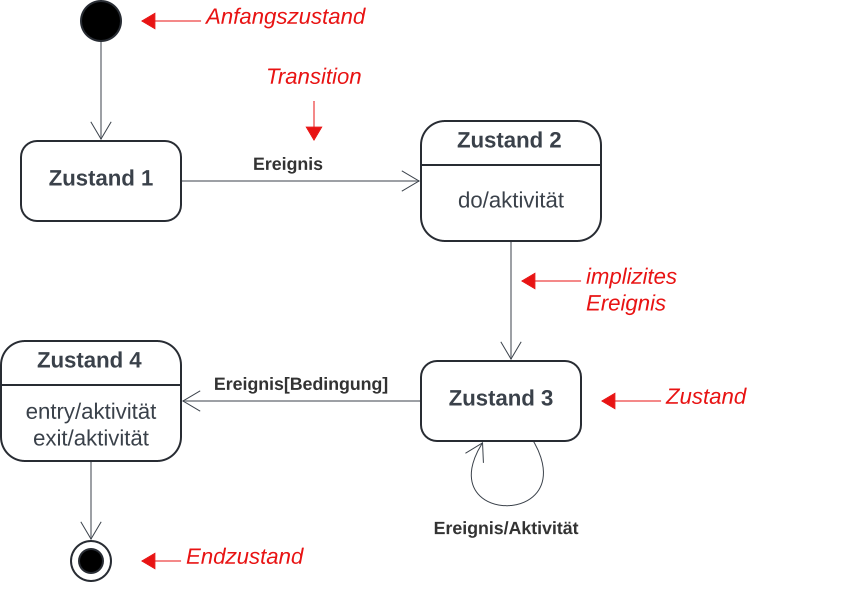
\includegraphics[scale=0.4]{part three/Zustandsautomaten/img/statechartdiagramnotation}
    \caption{Elemente eines einfachen Zustandsautomaten. Eine Transitionen wird durch ein \textbf{Ereignis} ausgelöst, das ein \textit{Signal}, ein \textit{Operationsaufruf} oder auch eine bestimmte \textit{Attributänderung} sein kann. (Quelle: in Anlehnung an \cite[90, Abb. 2.11-6]{Bal05})}
    \label{fig:statechartdiagramnotation-cc}
\end{figure}

\begin{figure}
  \centering
  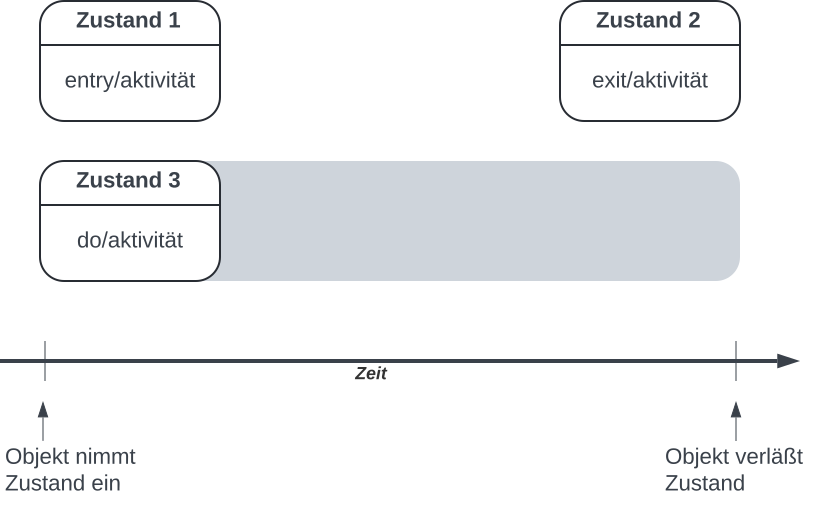
\includegraphics[scale=0.4]{part three/Zustandsautomaten/img/entryexitdo}
  \caption{Notationen für \textbf{entry}-,\textbf{exit}- und \textbf{do}-Aktivitäten sowie deren Dauer. Die \textbf{do}-Aktivität endet, wenn der Zustand verlassen wird. Die \textbf{entry}-Aktivität beendet sich von selbst. (Quelle: in Anlehnung an \cite[89, Abb. 2.11-3]{Bal05})}
  \label{fig:entryexitdo-cc}
\end{figure}

\begin{minted}[fontsize=\small]{java}
// Beispiel für eine Implementierung eines
// Parkscheinautomaten als Zustandsautomat in Java
class Parkscheinautomat {

  // zustände
  private final int BEREIT = 0;
  private final int ZAHLUNG = 1;
  private final int ABBRUCH = 2;
  private final int BELEG   = 3;

  // Zustand; wird initial beim Starten
  // des Automaten gesetzt
  private int zustand;

  // Methoden lösen Aktionen beim Eintritt
  // in die jeweiligen Zustände aus
  private int zahlung() {
    // verarbeiten
    // danach neuen Zustand zurückliefern...
    ...
    return BEREIT;
  }

   ...

  private void bereit() {
    while (true) {
      // eingabe überprüfen und
      // ggf. Zustandswechsel auslösen:
      // Zustand als Attribut setzen
      ...
    }
  }

  public void start() {
    zustand = BEREIT;

    while(true) {
      switch (zustand) {
        case BEREIT:
          zustand = bereit();
        // ... weiteres Verhalten
        ...
      }
    }
  }
}
\end{minted}